\chapter{Introduction}

\section{Figures}

Place your image in chapters/images folder. Refer \ref{fig:waterfall}
\begin{figure}
    \centering
    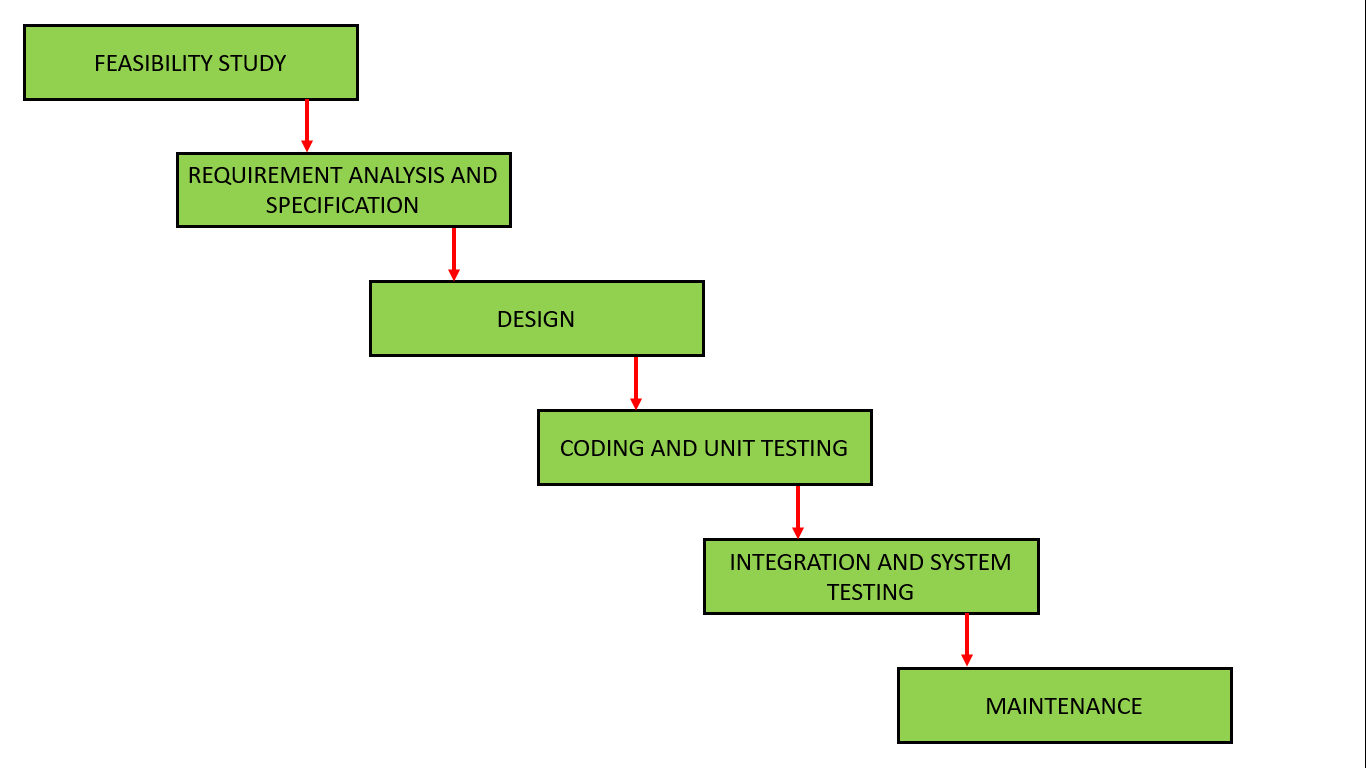
\includegraphics[scale=0.15]{chapters/images/waterfall.png}
    \caption{Various stages involved in the waterfall model}
    \label{fig:waterfall}
\end{figure}

\section{Code snippets}
Place your code snippets in codes folder. Refer \ref{fig:sample_code} 
\begin{figure}
    \begin{minted}{js}
function sample () {
    console.log("Sample code");
}
\end{minted}
    \caption{Sample function.}
    \label{fig:sample_code}
\end{figure}

\section{Tables}
\begin{table}[h!]
    \centering
    \begin{tabular}{l|l}
        A & B \\
        \hline 
        1 & 2 
    \end{tabular}
    \caption{Sample table}
    \label{tab:highlights}
\end{table}

\section{Abbreviations}
Create abbreviations in covers/abbreviations.tex file and refer them here using gls. Eg. Simple Abbr(\gls{sa})

\section{Footnotes}
You can add footnotes \footnote{Sample footnote}

\section{References}
Add BibTeX format bibliography entries in bib.bib and cite anywhere like this; \cite{sample_cite}